\documentclass[10pt, conference, compsocconf]{IEEEtran}
%\usepackage{CJKutf8}
\usepackage[UTF8]{ctex}
\usepackage{cite}
\usepackage{amsmath,amssymb,amsfonts}
%\usepackage{algorithmic}
\usepackage{graphicx}
\usepackage{textcomp}
%\usepackage{pythonhighlight}
\hyphenation{op-tical net-works semi-conduc-tor}

\begin{document}
	%\begin{CJK}{UTF8}{gbsn}

\title{基本共射级放大电路的仿真与探究}

%\author
%{\IEEEauthorblockN{Qilei Li}
%    \IEEEauthorblockA
%    {
%    EE\\
%    四川大学\\
%    成都, 中国\\
%    qilei.li@foxmail.com
%    }
%}

\author{
  薛昊辰,于宗玄,高浚哲,麻柯柯,胡潇丹
}

\maketitle

\begin{abstract}
本文详述了基本共射级放大电路的仿真结果,并结合当下背景,对集成电路的应用进行了分析。
\end{abstract}

\begin{textbf}
Abstract---In this paper
\end{textbf}

\IEEEpeerreviewmaketitle

\section{共射级放大电路的仿真}
%\begin{itemize}
%	\item	项目1
%	\item	项目2
%\end{itemize}
\begin{equation}
  I_{BQ}=\frac{V_{CC}-V_{BE}}{R_b}=\frac{12V-0.7V}{350k\Omega}=32.29\mu A
\end{equation}

\begin{equation}
  I_{CQ}=\beta I_{BQ}=50\times32.29\mu A=1.615mA
\end{equation}

\begin{equation}
  I_{EQ}=(1+\beta)I_{BQ}=1.647mA
\end{equation}

\begin{equation}
  \begin{split}
    V_{CEQ}&=V_{CC}-I_{CQ}R_C\\
    &=12V-1.615mA\times 4.2k\Omega=5.217V
  \end{split}
\end{equation}

\begin{equation}
  A_V=\frac{V_o}{V_i}=\frac{-\beta i_b(R_C//R_L)}{i_br_{be}}=\frac{-\beta(R_C//R_L)}{r_{be}}=-96.6
\end{equation}

\begin{equation}
  r_{be}=r_{bb'}+(1+\beta)\frac{26mV}{I_{EQ}}=1003.6\Omega
\end{equation}

\section{思政综述}
思政综述

\section{团队分工}
团队分工
\section{时间进度}
时间进度
\section{设计感想}
设计感想
\section{致谢}
感谢CCTV,感谢MTV,感谢所有TV

%\begin{figure}[h]
%	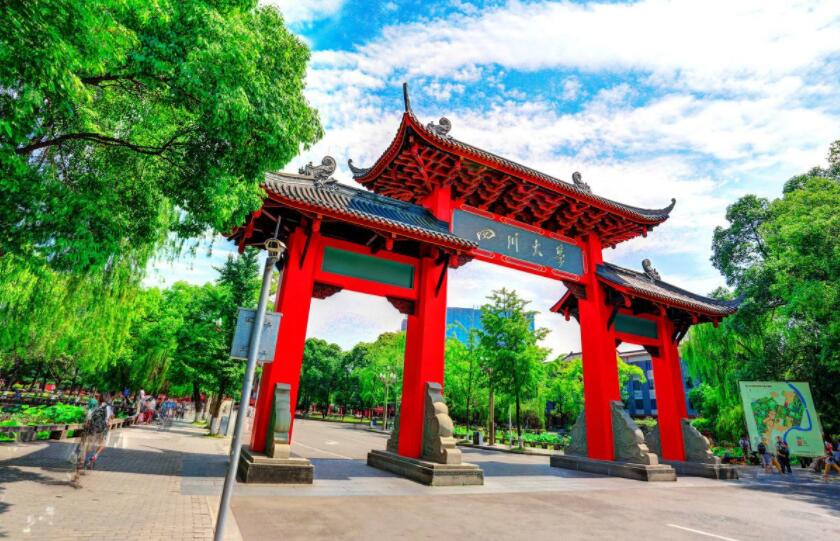
\includegraphics[width=8cm]{school.jpg}
%	\caption{school} 
%	\label{school}
%\end{figure}




\subsection{小节}
可以导入代码
%需要引用第三方库
%\begin{python}
%import numpy as np
%a = np.random.randn((5,5))
%\end{python}



\subsubsection{小小节}

\begin{equation}
  E= MC^2
\end{equation}


\begin{equation}
max(0,x)=\left\{
\begin{aligned}
0, \quad x \leq 0 & \\
1, \quad x > 0  &
\end{aligned}
\right.
\end{equation}

参考文献的引用:
\cite{yearbook2005china}

\bibliographystyle{IEEEtran} 
\bibliography{ref}   



%\end{CJK}
\end{document}
